% IMGAUG
% https://github.com/aleju/imgaug/blob/master/changelogs/v0.3.0.summary.md

\documentclass[thesis=B,english]{FITthesis}[2019/12/23]
% \usepackage[utf8]{inputenc} % LaTeX source encoded as UTF-8
\usepackage{minted}
% \usepackage{amsmath} %advanced maths
% \usepackage{amssymb} %additional math symbols
\usepackage{csquotes}
\usepackage{dirtree} %directory tree visualisation
\usepackage{xevlna}
% % list of acronyms
% \usepackage[acronym,nonumberlist,toc,numberedsection=autolabel]{glossaries}
\usepackage{glossaries} % glossaries
\makenoidxglossaries % glossaries
\usepackage{subfig}
\usepackage{graphicx}
% \usepackage{showframe}
% \usepackage{pdflatex}

\newglossaryentry{cpu}
{
    name=CPU,
    description={Central Processing Unit}
}

\newglossaryentry{gpu}
{
    name=GPU,
    description={Graphical Processing Unit}
}

\newglossaryentry{tpu}
{
    name=TPU,
    description={Tensor Processing Unit}
}

\newglossaryentry{cnn}
{
    name=CNN,
    description={Convolutional Neural Network}
}

\newglossaryentry{nn}
{
    name=NN,
    description={Neural Network}
}

\newglossaryentry{relu}
{
    name=ReLU,
    description={Rectified Linear Unit}
}

\newglossaryentry{api}
{
    name=API,
    description={Application programming interface}
}

\newglossaryentry{tf}
{
    name=TF,
    description={TensorFlow}
}

\newglossaryentry{xor}
{
    name=XOR,
    description={eXclusive OR}
}

\newglossaryentry{ml}
{
    name=ML,
    description={Machine Learning}
}

\newglossaryentry{sgd}
{
    name=SGD,
    description={Stochastic Gradient Descent}
}

\newglossaryentry{latex}
{
    name=latex,
    description={latex, mathematical writing language}
}

\newglossaryentry{tensor}
{
    name=tensor,
    description={is a generalization matrix}
}

\newglossaryentry{umap}
{
    name=UMAP,
    description={Uniform Manifold Approximation and Projection}
} % glossaries tenhle file si prozkoumej jak vypada

\counterwithin{listing}{chapter}

\newcommand{\tg}{\mathop{\mathrm{tg}}} %cesky tangens
\newcommand{\cotg}{\mathop{\mathrm{cotg}}} %cesky cotangens

\usepackage[style=iso-numeric,]{biblatex}
\addbibresource{!ref.bib}
\department{Department of Applied Mathematics}
\title{Deep learning for detection of defects in sewer CCTV}
\authorGN{Ondřej} %(křestní) jméno (jména) autora
\authorFN{Chládek} %příjmení autora
\authorWithDegrees{Ondřej Chládek} %jméno autora včetně současných akademických titulů
\author{Ondřej Chládek} %jméno autora bez akademických titulů
\supervisor{Mgr. Petr Šimánek}
\acknowledgements{I would like to thank my supervisor Mgr. Petr Šimánek for his guideance over the thesis and his helpful comments. I would also want to thank Dominik Chodounský for reading all the way through and finding grammar errors. Lastly I would like to thank to my girlfriend and family for their support during writing, without them this thesis would not be possible. Thank you all. }
\abstractCS{Práce je zaměřena na detekci poruch z~kamerové inspekce kanalizace. Cílem práce je vytvořit model hluboké neuronové sítě, která dokáže s~vysokou přesností určit, zda~je na daném snímku porucha v~kanalizaci či ne, a~ulehčit tak práci technikům, kteří by~jinak museli celý záznam analyzovat ručně. Natrénovaný model pro detekci chyb dosáhl přesnost na testovacím datasetu 99\%. Pro klasifikaci chyb navrhuji použít řešení pomocí dvou modelů, první by detekoval, jestli je obrázek vadný a nebo ne, druhý na základě obrázků označených jako vadné, by klasifikoval chyby. Pro detekci vad byl použit předchozí model. Přesnost klasifikace chyb byla 87\% na testovacích datech.}
\abstractEN{This thesis is focused on defect detection of~CCTV inspection of~sewerage. The aim is to create a model of deep neural network which can determine with high accuracy whether a given image contains defective canalization or not and thus to make it easier for technicians who would otherwise have to analyze the whole record manually. Trained model for defect detection managed to achieve 99\% performance on test set. For defect classification I suggest using two models, first would detect if given image contains defective canalization or not, second would classify which defect is present in the image. Previously mentioned model was used for defect detection. Classification accuracy on test set was 87\%.}
\placeForDeclarationOfAuthenticity{Prague}
\declarationOfAuthenticityOption{4} %volba Prohlášení (číslo 1-6)
\keywordsCS{detekce vad, klasifikace vad, hluboké učení, neuronová síť, přenos učení, Python, keras}
\keywordsEN{defect detection, defect classiffication, deep learning, neural network, transfer learning, Python, keras}
% \website{http://site.example/thesis} %volitelná URL práce, objeví se v tiráži - úplně odstraňte, nemáte-li URL práce

\begin{document}

% \newacronym{CVUT}{{\v C}VUT}{{\v C}esk{\' e} vysok{\' e} u{\v c}en{\' i} technick{\' e} v Praze}
% \newacronym{FIT}{FIT}{Fakulta informa{\v c}n{\' i}ch technologi{\' i}}

\begin{introduction}
    The deep convolutional neural networks are used mainly for image data. Different architectures created by scientists are publicly available so that anyone can use them for image classification. Defect detection belongs to the classification because it is a binary classification. Classification with very high precision could help technicians analyzing gigabytes of data. It could help allocate human resources into acquiring new footage or fixing defects. By defect image, I mean an image with a canalization defect present. Source data are in the form of video files. When technicians perform the CCTV inspection of canalization infrastructure, they have a device with a camera attached to a cable. Each video starts with information about where  the video is starts, which material the pipe is build from etc., but that information can also be found in the provided excel sheet. Because of the fact that source data are videos, the dataset is large and, for some part, excessive.
    
    The work is focused on finding such defects. The goal is to get a model with high precision of detection, which could speed up analyzing vast amounts of footage that water supply companies have from regular inspections.
    
    I chose this topic because I was curious about machine learning and artificial intelligence, and also I wanted to experience solving a real\babelhyphen{nobreak}life task.
    
    In the first chapter of the thesis, the theory of deep convolutional neural networks will be explained. Few image classification architectures will be introduced. In the next chapter, used tools and frameworks will be described.
    
    The goal of the theoretical part will be to explain convolutional neural networks, discuss their usability and modern state of the art architectures. Transfer learning will also be discussed because of its importance to model training. Dataset augmentation will also be mentioned, because of its value to unbalanced datasets.
    
    In the first part of the practical chapter, data acquisition from a video will be shown. Parameters of the dataset splitting into train, test and validation parts will be shown. The last part will be about model training in keras. Transfer learning will be used for image model training. At last, comparison between different architectures that can be transferred to the problem will be presented.
    
    The contribution of this thesis could be to ease the analysis of the canalization network for sewage companies. The model could say which parts of the video contain defective canalization and where to look for them. Because some parts of videos contain no defect, these parts could be skipped by a technician and he could focus only on those that need a decision about fixing. 
\end{introduction}


\chapter{Research}
In the past few years, scientists in computer vision made a lot of progress. Some of the computer vision tasks are image classification, object detection, and object segmentation. Image classification is when you are given a picture and you give the image label from a limited pool which you think the image belongs to. Object detection is a little more complicated. On the input, you also have an image, but you don't just classify the image, you have to detect all different classes inside the image and create bounding boxes around them. And the hardest task is object segmentation. The bounding box is not enough, you have to tell where exactly is the object in the image. The differences can be seen in Figure \ref{fig:cv_topics}

\begin{figure}
    \centering
    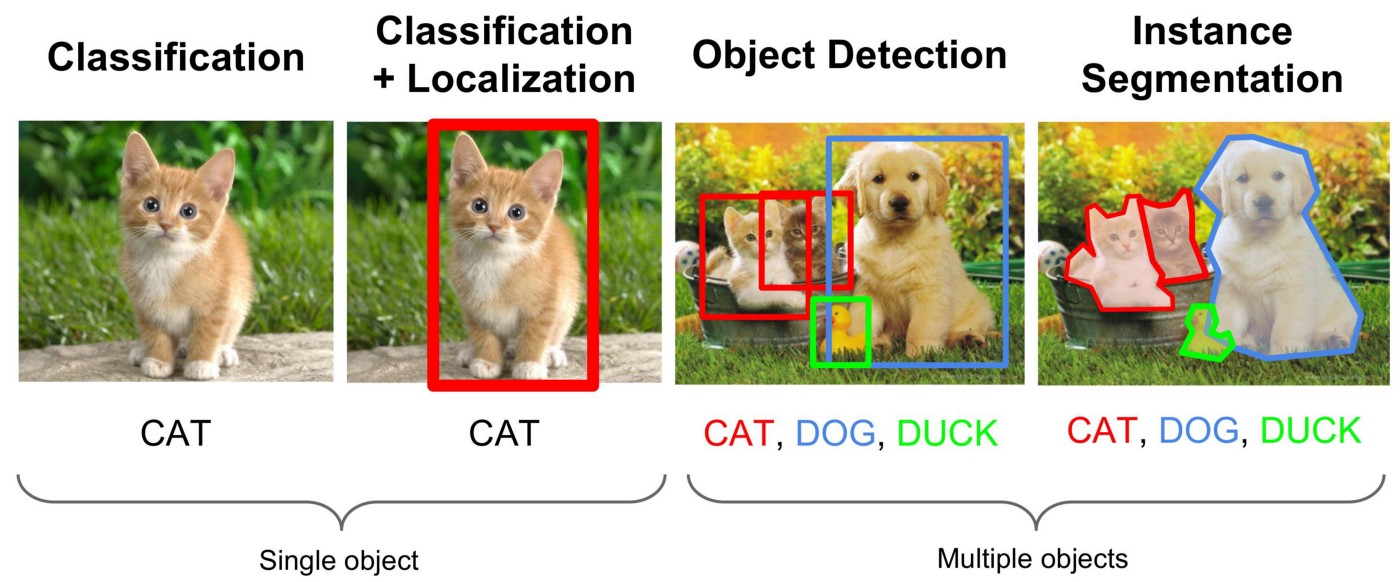
\includegraphics[width=0.8\textwidth]{cv_differences.jpeg}
    \caption[Image classification, object detection and instance segmentation]{Differences between image classification, object detection and object segmentation \cite{ouaknine_2018}.}
    \label{fig:cv_topics}
\end{figure}

However, this thesis is only focused on image classification since there is no need to actually find where the defect is, because there will be a human responsible for the decision, whether it is a serious issue and should be fixed as soon as possible, or it is some minor crack, that could be fixed next time when for example nearby pipes have to be replaced.

\section{Neural networks}
A Neural Network (\gls{nn}) is a computer system inspired by the human brain \cite{bengio2017deep}. It consists of neurons in layers that are connected between layers and algorithms to correct their input weights and activation function. \Gls{nn} can extract important features. 

\section{Convolutional neural networks}
A Convolutional Neural Network (\gls{cnn}) is a class of Neural Networks, most commonly used when inputs are images. Problem with Neural Networks is that they do not scale well to images because even in low res image, there is a lot of information (pixels). This can lead to Overfitting, more information about Overfitting can be seen in Section \ref{sec:overfitting}. Instead, we want to extract some features and pass those features to Neural Layer/s. As can be seen in Figure \ref{fig:conv_network} \gls{cnn}s are usually composed of four main operations:

\begin{figure}
    \centering
    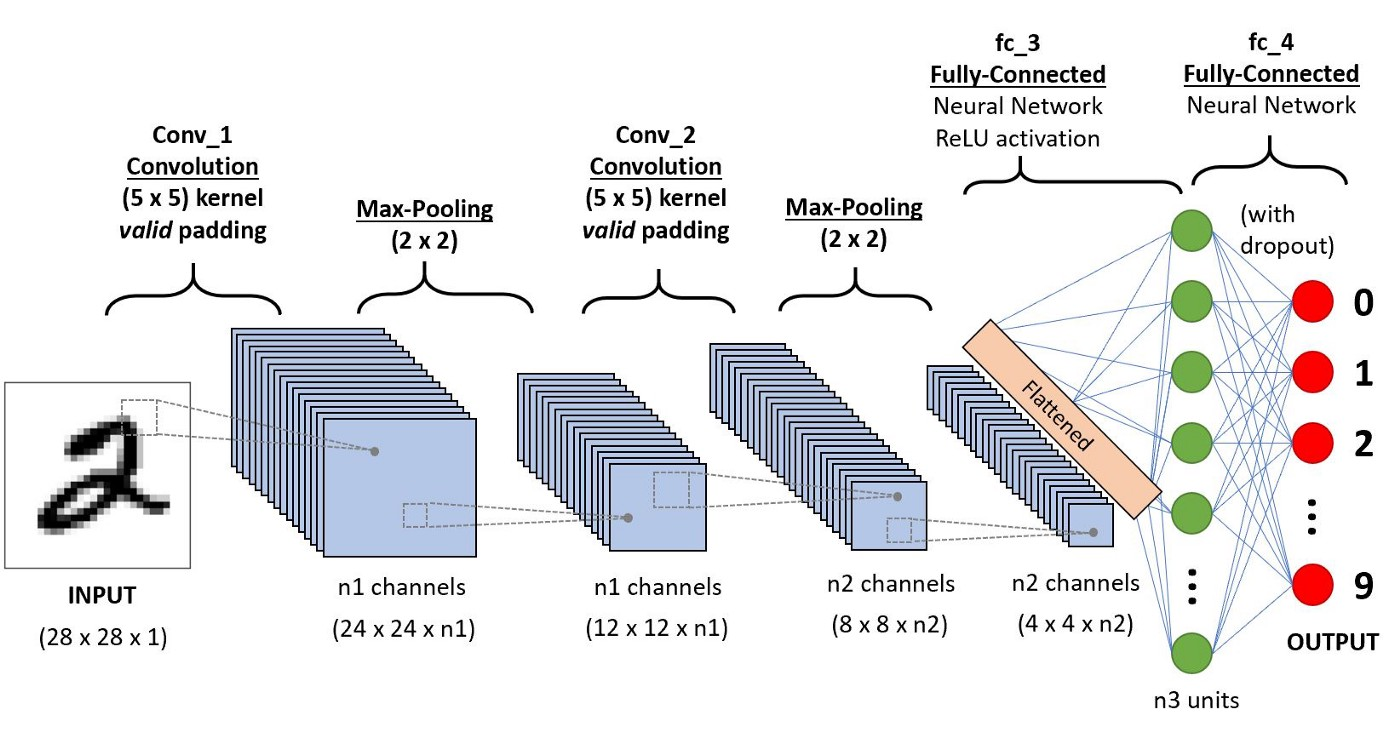
\includegraphics[width=.8\textwidth]{conv_network.jpeg}
    \caption[Convolutional Neural Network structure]{Structure of \gls{cnn}. \cite{saha_2018}}
    \label{fig:conv_network}
\end{figure}

\begin{enumerate}
    \item Convolution
    \item Non Linearity (\gls{relu})
    \item Pooling
    \item Dense Layer/s
\end{enumerate}

\subsection{Convolution}
    Convolution is a mathematical operation on two functions with real value arguments. You can imagine it as if you had some small matrix, often called a kernel, that is slid through the image, as can be seen in Figure \ref{fig:conv_operation}. On every valid position, you multiply weights with pixels and sum them together. Weights are sets of vectors that are initialized randomly and can be changed to provide better results (weight training). Mathematically it would be written as
    
    $$ (I * K)(i, j) = \sum_{m}\sum_{n} I(i+m, i+n)K(m, n) $$
    
    where $I$ is an input image, $K$ is the kernel, and $m, n$ are dimensions of the kernel \cite{bengio2017deep}. 
    
    \begin{figure}
        \centering
        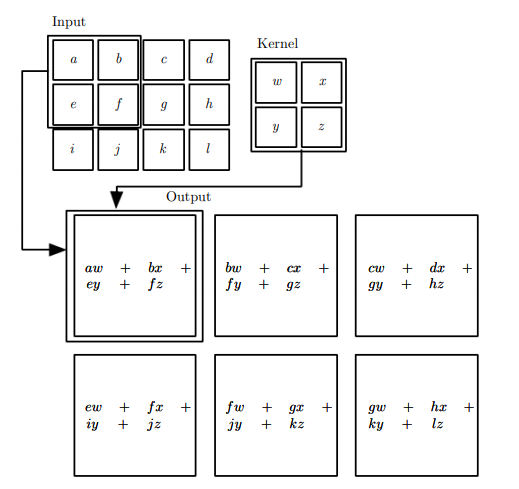
\includegraphics[width=\textwidth]{Convolution_operation.PNG}
        \caption[Convolution operation on 2D input]{Convolution operation on 2D input. Box is drawn to indicate how position of image is formed. In this case there is no zero\babelhyphen{nobreak}padding, often called \emph{valid}. This illustrates image shrinking in size after each operation \cite{bengio2017deep}.}
        \label{fig:conv_operation}
    \end{figure}
    
    Convolution in first layers of \gls{cnn} can detect features like edges. Imagine kernel size 3x3 with values like in Table \ref{tab:sample_kernel}. After the kernel is convolved with the image, there will be high values in places where vertical lines are. Similar can be done for horizontal and diagonal lines and for edges. This is how the first layers in \gls{cnn} typically work. And by combining the output of the first layers, we can detect shapes.

    \begin{table}[ht!]
        \centering
        \begin{tabular}{|c|c|c|}\hline
            -0.1    & 1.8     & -0.1\\\hline
            -0.5    & 1.9     & -0.8\\\hline
            -0.3    & 2.2     & -0.2\\\hline
        \end{tabular}
        \caption{Sample kernel}
        \label{tab:sample_kernel}
    \end{table}
    
     Every time convolution is applied, the image shrinks. This is why we can add padding. Padding is adding zero value rows/lines to the edges in order to preserve image size. Three types of zero\babelhyphen{nobreak}padding are worth mentioning. Firstly no padding can be applied, often called \emph{valid}. In this case, there is no change to the image, but the disadvantage is that the image shrinks every time we apply convolution. If the input image has width size of $n$ and kernel is size of $k$ than the output width will be size of $n - k + 1$, as can be seen in Figure \ref{fig:conv_operation}. This can be fixed by adding zero\babelhyphen{nobreak}padding every time image is convolved. Zero is used because there is nothing more, and we do not want to add some form of noise by using random numbers. This padding is called \emph{same} because dimensions stay the same. However, even in \emph{same} padding, some pixels have less impact on results than others. This lead to extreme case of \emph{full} zero\babelhyphen{nobreak}padding. In this case, every pixel, even corners are visited $k$ times for kernel size of $k$. Similarly, as in \emph{valid}, this leads to a change of input dimensions. Suppose again kernel size of $k$ and input width of $n$ than the resulting width will be $n + k - 1$. \cite{bengio2017deep}
    
\subsection{Non-linearity}
\begin{figure}
    \centering
    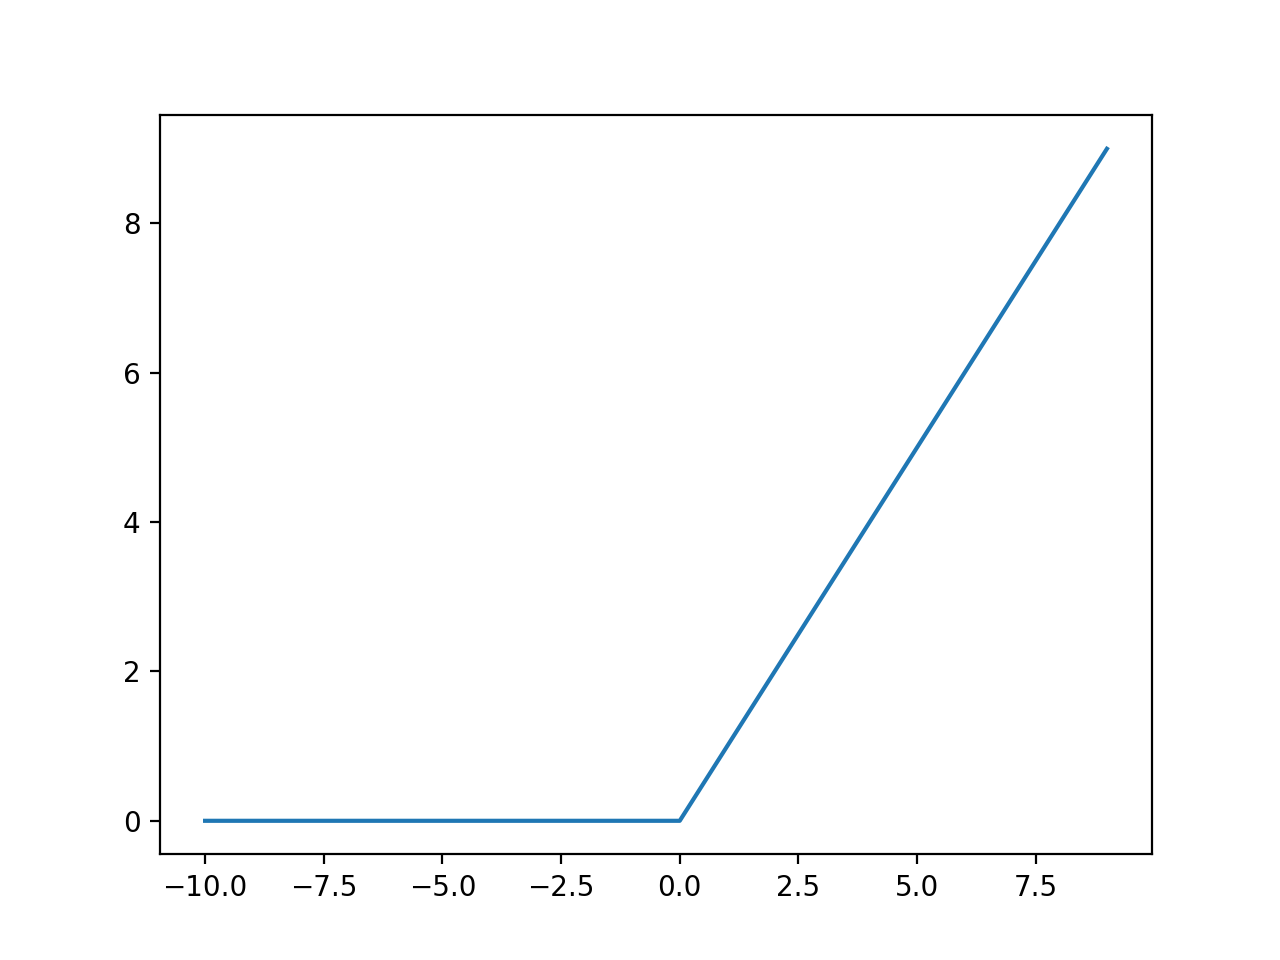
\includegraphics[width=0.8\textwidth]{relu.png}
    \caption[ReLU function]{ReLU function \cite{relu}}
    \label{fig:relu}
\end{figure}
    The use of hidden layers requires choosing activation function to compute values of hidden layers. Consider input vector $x_1, \ldots, x_n$ and weight vector $w_1, \ldots, w_n$, then the neuron output before the activation function will be $f(x, w) = x_1 \times w_1 + \ldots + x_n \times w_n$. Historically \gls{xor} problem taught us that linear activation function sometimes might not be enough. \gls{xor} is not solvable in linear space because there exists no function that could split it perfectly using only one line, as can be seen in Figure \ref{fig:xor}. This leads to use of non\babelhyphen{nobreak}linear functions. In modern Neural Networks the default recommendation is Rectified Linear Unit or \gls{relu} that is defined as $f(x) = max(0, x)$ as can be seen in Figure \ref{fig:relu}. \Gls{relu} is used because it is non\babelhyphen{nobreak}linear transformation but because it is nearly linear. This allows preserving generalization, something that linear models do well. Also, linear models are easy to optimize with gradient\babelhyphen{nobreak}based methods \cite{bengio2017deep}. Other activation functions can be for example  sigmoid: $f(x) = \frac{1}{1+e^{-x}}$ or TanH: $f(x) = \frac{e^x - e^{-x}}{e^x + e^{-x}}$. 
    
    \begin{figure}
        \centering
        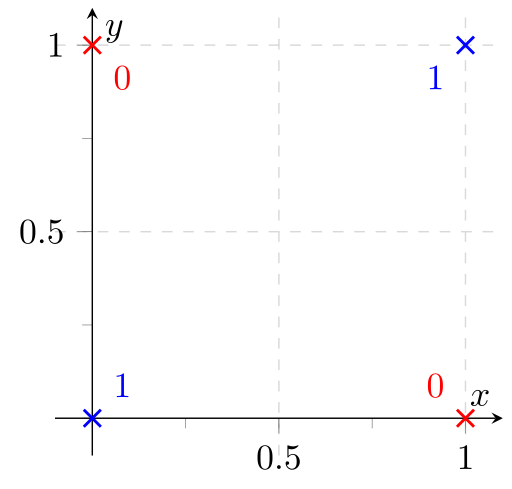
\includegraphics[width=.5\textwidth]{xor.png}
        \caption[XOR function]{\gls{xor} function.  \cite{thoma_2016}}
        \label{fig:xor}
    \end{figure}
    
\subsection{Pooling}
    Pooling is used to further modify the output of the previous layer. A pooling function replaces output at a certain location with summary statistics of nearby locations. The often\babelhyphen{nobreak}used \emph{Max pooling} reports maximum from a rectangular shape. Other variants exists and can be used, such as \emph{Average pooling}, \emph{L\textsuperscript{2} norm} or \emph{weighted average} \cite{bengio2017deep}. Max pooling example can be seen in Figure \ref{fig:maxpooling}
    
    \begin{figure}
        \centering
        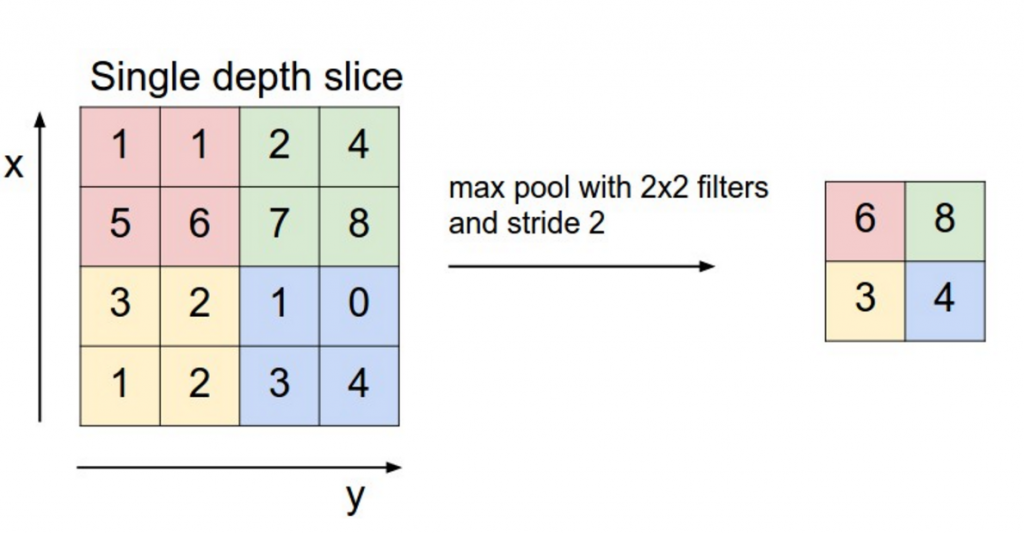
\includegraphics[width=.8\textwidth]{max_pooling.png}
        \caption[Max pooling example]{Max pooling example with 2x2 kernel and stride of 2. Stride refers to distance that the kernel is moved.  \cite{max_pooling_image}}
        \label{fig:maxpooling}
    \end{figure}
    
    Pooling helps with small translations making it more resistant to Overfitting (see Section \ref{sec:overfitting}) and decreases the number of parameters that are needed to train. This can be helpful if we care more about if the certain feature is present rather than feature location \cite{bengio2017deep}. For example, when detecting a car, pixel\babelhyphen{nobreak}perfect location of lights and side mirrors is not important, we just need to know that there is a light on each side, both sides have mirrors, there is a windshield.
    
\subsection{Dense}
    \gls{cnn} mainly contains 3 previously mentioned layers repeated several times to extract high level features. \emph{Dense} layer/s are able to transform those features into predictions. \emph{Dense} is a normal Multi Layer Perceptron layer that uses \emph{softmax} in output as activation function. \emph{Softmax} is mathematically written as:
    $$softmax(x)_{i}=\frac{exp(x_{i})}{\sum_{j=1}^{n}exp(x_{j})}$$  
    This function accepts real values and gives us values from $(0,1)$ and sum up to $1$. That is ideal for converting outputs of \gls{cnn} to probabilities.  

\section{Data preparation}
    When training artificial intelligence models, the first thing users have to do is to prepare data. Depending on the used model, it is necessary to apply some filter, standardize, or normalize. And we need to somehow measure the performance of the given model. We will use \emph{Test} error. \emph{Test} error is defined as the expected value of error on a new input \cite{bengio2017deep}. This error is what has to be as low as possible as well since models are created for predicting new data, not those that they have already seen. 

\subsection{Train and Test split}
    This can be tested by hiding some parts of the data. Usually data are split into \emph{Train} and \emph{Test} part. Test set is hidden from the \gls{cnn} while training. This gives us that new input we talked about earlier, and thus test error can be computed. The train and the test datasets should be split so that the distribution of classes in both datasets stays relatively the same. This can be achieved with a stratified split. But when optimizing hyperparameters (see Section \ref{sec:hyperparameters}), the test set might not be enough since we would optimize for the test set, thus losing generalization. More about generalization can be seen in Section \ref{sec:overfitting}. 

\subsection{Validation}    
    By adding a validation set, we can easily hide the test set for later use and tune hyperparameters on the validation set. This gives us new input for hyperparameter tuning so we can adjust them for good performance on the validation set, and after everything is set, the model can be tested against the test set for evaluation purposes.
    
    Another technique that can be used is cross\babelhyphen{nobreak}validation. This technique splits data into train and test, and after learning, it evaluates results on the test set. Then a different test set is chosen, the model is trained again from scratch and evaluated. This is repeated until the whole dataset is covered by different test sets. When finished, we have results that could represent the whole dataset \cite{browne2000cross}.

  
\subsection{Normalization}
    Normalization is an important scaling mechanism that allows them to work properly. By using normalization, we can achieve an easier function landscape, which gives better results, because finding minimum is easier. Also, by simplifying the function landscape, the model can learn quicker because it does not have to explore different local minimums. Without normalization, the model might not even converge \cite{bengio2017deep}.
    
    Standardization is often used as a normalization technique since it proved very effective. It creates an environment where each feature has zero mean and variance of one. Standardization can be written as:
    $$x^{'} = \frac{x - \Bar{x}}{\sigma}$$
    where $x$ is the original feature vector, $\Bar{x}$ is mean of a feature vector and $\sigma$ is the standard deviation.

\section{Model Training}
    Models are usually trained in epochs with some form of gradient descent used. Epoch represents one full training cycle over the entire dataset. Gradient Descent can be used together with momentum to achieve faster learning rates.

\subsection{Loss Function}
    But first, we need to talk about loss function. Loss function can be described as a function that measures how well the model performed or how much it deviated from the optimal solution. It gives the model information on how well it performed and how to continue the training process. Because of the usage of Gradient Descent, this function has to have a minimum in cases where the model is best and increases if the model has a bad performance. The typical loss function for the categorical problem is Categorical Cross\babelhyphen{nobreak}Entropy. This is written as
    $$L(x, y, \theta) = - log(p(y|x;\theta))$$
    
    where $x$ is an element of train set, $y$ is target associated with $x$ and $\theta$ are parameters in \gls{nn}. This function is minimized, when $p$ for the correct class is $1$, so it meets the requirements mentioned earlier. Other loss functions are e.g., Mean Squared Error for Regression problems and Binary Cross\babelhyphen{nobreak}Entropy for Binary problems.
    

\subsection{Gradient Descent}
    Training requires some form of optimization of loss function. Since the goal is to minimize it, the best way how to do it in theory would be to calculate gradient and after that move against it. Gradient descent for $m$ train examples can be written as:
    $$g = \Delta J(\theta) = \frac{1}{m}\sum_{i=1}^m\Delta_{\theta}L(x^{i}, y^{i}, \theta)$$
    
    Where $\Delta_{\theta}L(x^{i}, y^{i}, \theta)$ is calculated gradient for $x^i$ element. Gradient downhill can be used using following equation:
    $$\theta \leftarrow \theta - \epsilon g$$
    where $\epsilon$ is learning rate \cite{bengio2017deep}.
    
\subsection[SGD and Batch Training]{Stochastic Gradient Descent and Batch training}\label{sec:sgd}
    Since training has to be done in real\babelhyphen{nobreak}world conditions and real\babelhyphen{nobreak}world limits us with how much resources we have, it is not a bad idea to figure out how to overcome those limitations. Almost all of the deep learning is powered by an algorithm named Stochastic Gradient Descent (\gls{sgd}). Training a large amount of data is computationally difficult, $O(m)$ with gradient descent. As the training set grows, it would take too long for one gradient step to take place. The insight of \gls{sgd} is that the gradient is an expectation. This expectation can be approximated by using small set of samples called Minibatch $B = \{x^{(1)},\ldots, x^{(m^{'})}\}$ drawn uniformly from training data. The batch size $m^{'}$ is typically some relatively small number. Also, $m^{'}$ is usually fixed, even if the dataset grows. The estimate of the gradient is \cite{bengio2017deep}:
    $$g = \frac{1}{m^{'}}\Delta_{\theta}\sum_{i=1}^{m^{'}}L(x^{i}, y^{i},\theta)$$ 
    
    and the stochastic gradient descent algorithm follows the estimated gradient downhill in the same way as gradient descent does. 
    
\subsection{Momentum}
    While Stochastic Gradient Descent is powerful enough for learning, it can sometimes be slow. The method of momentum was designed to accelerate learning in some cases where the gradient is consistent but small. The momentum algorithm accumulates an exponentially decaying average of past gradients and continues to move in their direction \cite{bengio2017deep}.
    
    The momentum algorithm introduces a variable $v$ that can be imagined as velocity or the direction and speed that parameters move in parameter space. The velocity is set to exponentially decaying average of the negative gradient. A hyperparameter $\alpha$ determines the decay rate. Velocity is calculated as:
    $$v = \alpha v - \epsilon\Delta_{\theta}(\frac{1}{m} \sum_{i=1}^m L(x^i, y^i, \theta)$$
    and weights are updated in the following fashion:
    $$\theta = \theta + v$$
    The larger $\alpha$ is relative to $\epsilon$, the less the velocity decays, and the more previous gradients affect the learning rate. This can also help from escaping local minimums, which are not desirable, because of worse results \cite{bengio2017deep}.

\subsection{Overfitting, Underfitting and Generalization} \label{sec:overfitting}
    
\begin{figure}
    \centering
    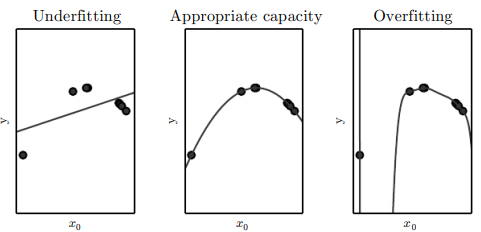
\includegraphics[width=.8\textwidth]{underfitting_overfitting.PNG}
    \caption[Underfitting and Overfitting]{Differences between Underfitting, Appropriate fit and Overfitting. Samples synthetically made from the quadratic polynomial. On the left graph, we can see that linear function cannot capture the curvature of data. The middle shows us a perfect fit that would generalize well on the chosen data since we know that source is a quadratic function. The right part of the figure shows us Overfitting because this model has a polynomial degree of 9. This model clearly does not represent data well since it generalizes poorly. \cite{bengio2017deep}}
    \label{fig:overfit}
\end{figure}
    Overfitting and Underfitting are tightly connected to bias and variance. Bias refers to how much the model ignores training data. Variance tells us how much the model is affected by training data. Underfitted models tend to have low variance and high bias, and the model has too large training error. Overfitted models, on the other hand, have high variance and low bias, relying too much on training data and thus not generalizing well. Also, noise can change the model so much, that test error rises quickly. The relation between Underfitting, Right fit and Overfitting can be seen in Figure \ref{fig:overfit}. Generalization means how well the model performs on new data. Often when the model is Overfitted, that model can easily differentiate labels from the train set, but on validation or test set, it fails with a noticeable difference. 
    
\subsection{Hyperparameters} \label{sec:hyperparameters}
    The model can have a lot of parameters. In Machine Learning parameters that are set before the model is trained, are called hyperparameters. Those can be learning rate of gradient descent, different methods of descending, also called Optimizers, number of Convolutional, Pooling and Dense layers, number of Neurons in Dense layer, etc. The model cannot change those parameters, although they can be set automatically using methods like Grid Search. Grid Search can be used if we do not know exactly how to set a given hyperparameter, but we might have a suspicion that it might be inside an interval. Training is then done several times, each time with different hyperparameters set. This can be done even for a combination of hyperparameters, but exploration time grows exponentially, because every time we want to automatically find another value, we add another dimension. Because of that, most hyperparameters have a default value, that performed well on most tasks. Another method suggested \cite{bengio2017deep} is to set space exactly like in Grid Search, but search randomly. Grid Search can miss some values, that random search could find. 

\section{Regularization}
    In \gls{ml}, there is an incentive to reduce test error, sometimes at the expense of training error. These strategies are known as regularization. There are many forms of regularization, in this thesis, two of them will be used, and that is \emph{Data Augmentation} and \emph{Early stopping}. Using some form of regularization can lead to improved performance on the test set.

\subsection{Data Augmentation}
\begin{figure}
    \centering
    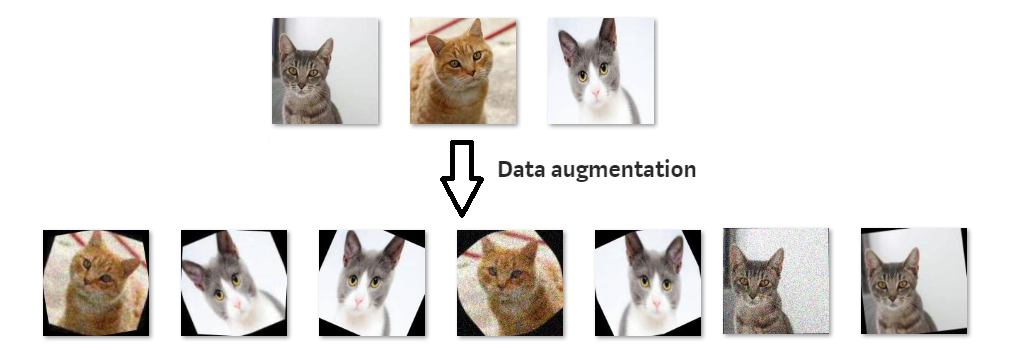
\includegraphics[width=\textwidth]{image_augmentation.png}
    \caption[Data augmentation example]{Data augmentation example \cite{himblot_2018}}
    \label{fig:augmentation}
\end{figure}
    Data augmentation is process when dataset is modified in order to create small translations in images. If model was trained, for example, only on precise camera movement, in the future it could not be able to process correctly footage, that was not precise. This helps with generalization, when model is deployed.

    Synthetic data can be created using \emph{Data Augmentation}. The only thing is that synthetic images have to be realistic. The image can be flipped vertically, but not horizontally since gravity has to apply. Water cannot flow on top unless the camera was flipped, but let's not consider that. A small change in distortion, skewing, rotation, and shearing can be done. Random cropping is not a good idea since it could create different classes, in my example, an annotated defect might not be present anymore. Some examples of Data Augmentation can be seen in Figure \ref{fig:augmentation}.
    
    In the case of an unbalanced dataset, which is typical in most of \gls{ml} tasks, new images can be synthetically created in underbalanced classes and/or some images can be deleted from class, which has the majority. Unbalanced datasets are a problem because the model can quickly learn that high probability for one class can give high accuracy. Data Augmentation can help fight that.
  
  
\subsection{Early Stopping}
When training models, often a steady decrease in train error can be seen, but that is not true for the validation error. Validation error declines in first epochs, but after some time, it can grow as can be seen in Figure \ref{fig:early_stopping}. This means we can obtain a model with a better validation error and hopefully better test error by returning to some previous stage where validation error was the lowest. Every time validation error improves, a copy of the model with parameters is stored. When the training algorithm terminates, the returned model is that with the lowest validation instead of the latest one \cite{bengio2017deep}. Learning terminates when no parameters have improved over some time, which is often called \emph{Patience}.

\begin{figure}
    \centering
    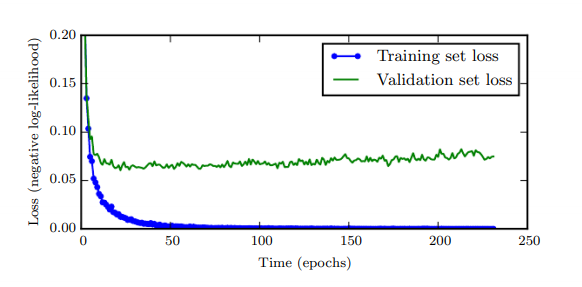
\includegraphics[width=\textwidth]{Early_stopping.PNG}
    \caption[Learning curve showing how test and validation error behaves]{Learning curve showing how validation loss drops and after that slowly rises. Training error on the other hand slowly approaches zero \cite{bengio2017deep}.}
    \label{fig:early_stopping}
\end{figure}


\section{Transfer Learning}
    Transfer learning allows us to use models previously trained on a similar task and convert it to a slightly different task. For example, a model trained on computer vision benchmark ImageNet (see \ref{sub:imagenet}) can be transferred to perform different computer vision tasks. By removing the last layers that serve as a classification layer and adding own layers specific for the problem that is being solved, training time can be reduced, and accuracy boosted \cite{bengio2017deep}. It is a good idea to still train a few of the last layers to specialize more transferred network.

\subsection{ImageNet dataset}\label{sub:imagenet}
    ImageNet is a dataset containing 1000 classes and over million of annotated images \cite{imagenet_stats}. This dataset is important in Computer vision as it serves as a baseline for transfer learning. Publicly available architectures with weights that were trained on ImageNet can be used as a baseline for different computer vision tasks. In 2012 network called AlexNet achieved top 1 and top 5 (see \ref{sub:topkek}) error rate on test set 37.5\% and 17\% \cite{alexnet}.
    
\subsection{ImageNet state of the art}
    Since creation of ImageNet, there were many competitors and improvements. AlexNet was already discussed so lets take look at more recent results. In 2014 network \emph{VGG19} achieved 25.5\% error rate on test set \cite{vgg}. Few year later \emph{ResNet-152} architecture showed with 19.4\% error rate \cite{resnet152}. Today the state of the art is \emph{FixEfficientNet-L2} with 11.5\% error rate \cite{fixefficientnet}.  

\section{Result Evaluation}\label{sub:topkek}
Models can be evaluated using different methods. Accuracy is used for categorical and binary problems. If the model says something, we want to believe that it is true. Accuracy can be computed as:

$$acc = \frac{n_{correct}}{n_{total}}$$

Where $n_{correct}$ is the number of correctly predicted images and $n_{total}$ is the number of total images.

But sometimes the problem is too hard, that even experts in that field argue what the right answer is. Sometimes \gls{ml} model can be undecided, too, so the first $k$ elements can be used as the evaluation method. This is like accuracy, but some form of tolerance is introduced. In the case of large class datasets like ImageNet, sometimes the right answer can be in second to $k$\babelhyphen{nobreak}th place. If it is, then in TOP k accuracy, it is considered correct. Although $k$ should not be a high number in regards to the number of classes, that would devaluate results and give almost 100\% results every time. But for example, TOP 5 accuracy is used in ImageNet \cite{alexnet, vgg, resnet152} because it has 1000 classes inside and gives result some form of tolerance to undecidedness.

We might be also focusing on false positivness or negativness. Precision is fraction of detections reported by the model that were correct or mathematically as $p = \frac{t_p}{t_p + f_p}$ where $t_p$ is true positive and $f_p$ is false positive. Recall is on the other hand fraction of $t_p$ that were detected or $r = \frac{t_p}{t_p + f_n}$. Usually we want to combine both of those values and that is called $F$-score. $F$-score can be calculated as $F = 2\times\frac{p \times r}{p + r}$ \cite{bengio2017deep}.

\chapter{Used Tools}

\section{Python}
Python is a programming language created by Guido van Rossum first released in 1991. Python was designed to be highly extensible. Thus there are many modules almost for anything. This can be used to ease the process of Data Preprocessing and Machine Learning. Some of those libraries use C/C++ backend to speed up the process of computing \cite{numpy_2020, google_brain_2020}.

\section{Jupyter and Google Colab}
Project Jupyter is a tool that enables writing code in blocks. Those blocks can be run out of order, making hyperparameter tuning easier. Google took it further with their Colab product. Users have features of typical Jupyter Notebook with the added value of free \gls{gpu}s/\gls{tpu}s. Also, it works like any other Google cloud service, so it can be shared easily between multiple users. This is great for people working remotely from each other as git does not offer real time code sharing, which is useful e.g., for teachers so they can check the code of their students.

\section{OpenCV}
OpenCV is an Open\babelhyphen{nobreak}Source Computer Vision Library \cite{opencv_2020} under the BSD license. It contains Python, C++, and Java interfaces and has high computational efficiency. OpenCV has a lot of features, but in this thesis, only video stream input will be used for collecting samples. 

\section{TensorFlow and Keras}
TensorFlow (\gls{tf})is an open\babelhyphen{nobreak}source framework for machine learning. It can be used on different platforms (\gls{cpu}s, \gls{gpu}s, \gls{tpu}s). Created by Google Brain team from Google AI organization and is fully supported on Google Colab. \gls{tf} has multiple levels of abstraction, and users can choose the right for their needs \cite{google_brain}. 

Keras, on the other hand, is a high\babelhyphen{nobreak}level \gls{api} for TensorFlow. Like \gls{tf}, keras is also open\babelhyphen{nobreak}source. It was developed with a focus on enabling fast experimentation. It is easier to prototype \gls{nn} in Keras since adding layers is as simple as one method. Keras also support Theano \cite{theano} and CNTK \cite{microsoft_2020} backends, so the user can switch if he desires to. User also can choose if he desires to train on \gls{cpu}, \gls{gpu} or \gls{tpu}. Two types of models exist in keras:

\begin{enumerate}
    \item Sequential
    \item Functional
\end{enumerate}

The Sequential model is a series of linear layers on top of each other. It can serve as a basic but powerful model for almost anything. The functional model was created to allow easy creation of complex models, allowing multiple inputs and outputs and it can also do skip connections, put layers in non\babelhyphen{nobreak}linear order and many more, which sequential model cannot do. For purpose of this thesis \emph{Sequential} model will be enough \cite{keras_main, keras_sequential, keras_functional}.

\subsection{Sequential example}
Creating a model in keras sequential is straightforward. User can either pass list of layers imported from \mintinline{python}|keras.layers| module or instantiate model and use \mintinline{python}|add()| method with instantiated layer. See Listing \ref{lis:seq_example}. After user\babelhyphen{nobreak}defined desired architecture, the model needs to be compiled. There the user can specify loss function, optimizer and metrics, and other parameters, but those three are the most common ones. Some examples can be seen in Listing \ref{lis:seq_example_compile}

\begin{listing}
    \begin{minted}{python3}
        from keras.models import Sequential
        from keras.layers import Dense, Activation

        model = Sequential([
            Dense(32, input_shape=(784,)),
            Activation('relu'),
            Dense(10),
            Activation('softmax'),
        ])
        
        # Or by using add method
        model = Sequential()
        model.add(Dense(32, input_dim=784))
        model.add(Activation('relu'))
    \end{minted}
    \caption[Keras Sequential example]{Keras Sequential example \cite{keras_sequential_example}.}
    \label{lis:seq_example}
\end{listing}


\begin{listing}
    \begin{minted}{python3}
        # For a multi-class classification problem
        model.compile(optimizer='rmsprop',
                      loss='categorical_crossentropy',
                      metrics=['accuracy'])
        
        # For a binary classification problem
        model.compile(optimizer='rmsprop',
                      loss='binary_crossentropy',
                      metrics=['accuracy'])
        
        # For a mean squared error regression problem
        model.compile(optimizer='rmsprop',
                      loss='mse')
    \end{minted}
    \caption[Model compiling examples]{Model compiling examples \cite{keras_sequential_example}.}
    \label{lis:seq_example_compile}
\end{listing}

When a model is compiled, it can finally be trained. Model training is done by calling \mintinline{python}|fit()| method. The user has to specify the source of the train data. Optionally the number of epochs can be specified. In the case of batch training (see Section \ref{sec:sgd}), steps per epoch can be changed, mostly to match one epoch with the whole dataset. In case of \emph{Cross\babelhyphen{nobreak}Validation} validation dataset and validation steps has to be provided. 


\chapter{Realization}
This chapter describes the training process from preprocessing to evaluation and possible deployment. Also, different architectures will be compared to see which one did the best. For preprocessing, \mintinline{bash}|jupyter notebook| was used because of its ability to run code cells out of order, reproducible outputs and easy exportability. Notebooks can be viewed on enclosed medium (Appendix \ref{app:CD_content})

\section{Data preprocess}
When encountering new data to train models, the programmer needs to do several procedures. First, data have to be explored in order to maybe find wrongly tagged instances and to get a general idea of what you are dealing with. This can help you with tasks that will come up next in the training phase. Also, it is a good idea to create a baseline, which you want to surpass or at least get close to since no model can generally achieve 100\% accuracy on test data. 

\subsection{Dataset exploration}
Dataset is called \emph{Sewer scanning CCTV footage} \cite{wessex_dataset}. Data were in the form of video files, defects were marked in an excel sheet, so data need to be sorted in classes separately. I was using OpenCV to extract images and pandas to search if an image contains a canalization defect or not created a heavily unbalanced dataset. Data were extracted using a jupyter notebook, that was provided by my supervisor and is attached on the enclosed medium \cite{mvi_extraction_notebook}. The material of each photo was also included in the excel sheet, so a decision was made to exclude materials that do not have either defect or healthy image. That lead to 15 defect classes plus one class for healthy images. The number of images was around 25 000, half of them representing images of healthy canalization and the other half images containing the defect. From now on, If I mention a healthy image, I mean an image with no canalization defect and for if I mention defect image, that means there is a canalization defect present in the image.

\begin{figure}

\subfloat[No Defect]{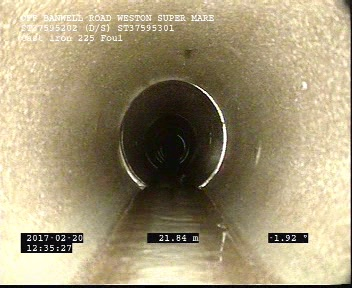
\includegraphics[width = 0.25\textwidth]{Healthy.jpg}}
\subfloat[Label DEG]{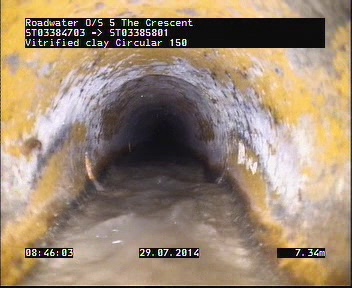
\includegraphics[width = 0.25\textwidth]{DEG.jpg}}
\subfloat[Label CL]{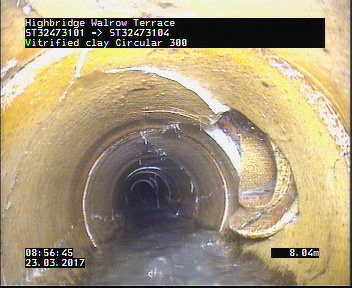
\includegraphics[width = 0.25\textwidth]{Crack_CL.jpg}}
\subfloat[Label RF]{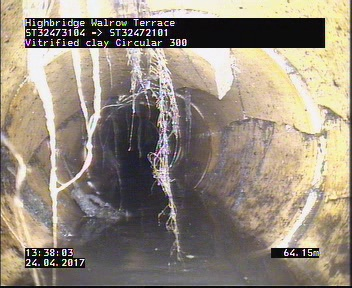
\includegraphics[width = 0.25\textwidth]{RootRF.jpg}}
\caption[Image examples]{Image Examples. First image contains no defect at all. Second image is some minor degradation. Third image has pipe cracked. Fourth image has a root of a plant growing through the canalization pipe. }\label{fig:e}
\end{figure}


We wanted to do two experiments. First was how a good model could be created to classify only to binary classes if the image contains a defect or not. The second task was to predict which class image belongs to. This could be done using either model with 16 classes, one for healthy and the rest for defect classes, or by combining the previous model, which would detect if a given image contains a defect or not and if it had defect present, the second model could be used to classify the type of the defect. According to Wessex Water, if any model could be as 80\% efficient as humans are, there might be a contract to implement the given model in the production environment \cite{wessex_challenge}.

\begin{figure}
    \centering
    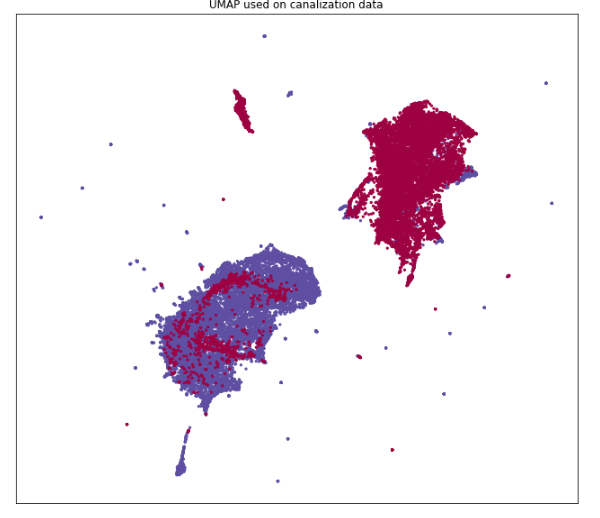
\includegraphics[width=\textwidth]{umap.PNG}
    \caption[\gls{umap}]{\gls{umap} used on dataset. Red dots represent images with canalization defect, purple dots images with no defect. Features were extracted on VGG16 model with weights from ImageNet.}
    \label{fig:umap}
\end{figure}

While exploring the dataset, we used Uniform Manifold Approximation and Projection (\gls{umap}). \gls{umap} can help with seeing the latent features of data \cite{lel2018umap}. If we manage to extract features of image, for example, by using \gls{cnn} without top Dense layers, we can feed those features into \gls{umap}. This can help with imagining how computers view a given problem. The model used for feature extraction was VGG16 without top layers since this model was trained on images and can do feature extraction in its convolutional part. Results were surprising, since for binary classification without training, there was an almost clear separation (images were clustered in two clusters) between data in 2D space for predicting which image belongs to which class. Results can be seen in Figure \ref{fig:umap}. What does it mean? We believe that VGG could be a good model for this task and will be used for establishing a baseline before any hyperparameters are changed.


\subsection{Train, Validation and Test split}
After the data has been explored, split into train, validation, and test samples have to be done. Function \mintinline{python}|train_test_split| from \mintinline{python}|scikit-learn| was used together with stratify split option. 20 \% of all data was allocated for the testing set, and another 20\% of train data were allocated to the validation dataset. Stratified split was used to ensure the presence of minor classes in each set. 

In keras there is a class \mintinline{python}|ImageDataGenerator| with a method, which loads images with labels depending on how they are structured inside a defined folder, named  \mintinline{python}|flow_from_directory|. It works like any other python generator, so it does only load a specified number of images at a time to save memory. This defaults to 32 but can be changed. Because of that, images had to be saved in a specific structure that can be seen in Fig \ref{fig:data_structure}. 

\begin{figure}
    \dirtree{%
        .1 test.
        .2 Class1.
        .3 Image1.
        .3 Image2.
        .3 \vdots.
        .2 Class2.
        .3 Image1.
        .3 \vdots.
        .2 \vdots.
        .2 Class$N$.
        .1 train.
        .2 Class1.
        .2 \vdots.
        .1 validation.
        .2 Class1.
        .2 \vdots.
    }
    \caption[Data structure]{Data structure required by \mintinline{python}|ImageDataGenerator|. Each set has to have same amount of classes in subfolders and images are put into class subfolders}
    \label{fig:data_structure}
\end{figure}

\subsection{Image preprocessing}
\mintinline{python}|ImageDataGenerator| also allows to specify preprocessing function, so data can come already preprocessed. For each architecture keras has a function, the user only has to import it and specify in the constructor of the class. This is enough to handle all preprocessing functions for any \gls{ml} architecture available on keras. Usage can be seen in Listing \ref{lis:imagedatagen}.

\begin{listing}
    \begin{minted}{python}
datagen = ImageDataGenerator(preprocess_input) 

train_generator = datagen.flow_from_directory(
    '/content/train',
    target_size=(224, 224),
    batch_size=BATCH_SIZE,
    class_mode='categorical',
    shuffle=True)

validation_generator = datagen.flow_from_directory(
    '/content/validation',
    target_size=(224, 224),
    batch_size=BATCH_SIZE,
    class_mode='categorical',
    shuffle=False)

test_generator = datagen.flow_from_directory(
    '/content/test',
    target_size=(224, 224),
    batch_size=BATCH_SIZE,
    class_mode=None,
    shuffle=False)

    \end{minted}
    \caption[Example usage of ImageDataGenerator ]{Example usage of \mintinline{python}|ImageDataGenerator|. Object is initialized with preprocessing  function that will be applied to each image. Parameter \mintinline{python}|shuffle| is set to True in train dataset to increase probability of multiple classes in one batch. Value \mintinline{python}|target_size| must match with input layer of \gls{cnn}.}
    \label{lis:imagedatagen}
\end{listing}

\section{Data Augmentation}
Dataset was augmented in order to create a less unbalanced dataset and to improve the generalization potential of the model. For augmentations package \mintinline{python}|Augmentor| \cite{augmentor} was used. It offers many transformations together with a pipeline, where the user specifies the probability of given transformation happening and boundaries of transformation. After that method \mintinline{python}|sample()| can easily create any number of images. This library was used because of its production\babelhyphen{nobreak}like pipeline, which can easily create many different augmentations on one image, and if the image was, for example, skewed, it could automatically crop the image, so it contains minimum or none of a synthetically added information (i.e., black parts). This is helpful in preserving natural parts of the image. 

A new dataset with 500 augmented images for each class was created. In order to create a less unbalanced training dataset, only classes with less than the number of augmented images were chosen for Augmentation. This proved very helpful while training since it gave better results than without Augmentation. It was probably because the training set was more balanced than in the beginning, and the model could not have good training results while having major class dominating output probabilities. If not mentioned otherwise, when training categorical data, this dataset will be used. 

\section{Model Training}
Model training was done using google colab and their free \gls{gpu}s. If not specified exactly, adam optimizer with default parameters will be used. Learning rate defaults at $1 \times 10^{-4}$, beta\_1 and beta\_2 defaults to $0.9$ and $0.999$ respectively. Epochs will be set to 30, but Early Stopping with patience equal to 4 might prevent full 30 epochs from finishing. Early Stopping is a callback that returns the best model if, for some amount of time, known as patience, the defined evaluation parameter has not improved. Setup of Early Stopping can be seen in Listing \ref{lis:early_stopping}.

\begin{listing}
    \begin{minted}{python}
    
early_stopping = callbacks.EarlyStopping(monitor='val_loss',
    min_delta=0,
    patience=4,
    verbose=1,
    mode='auto',
    restore_best_weights=True
)
    \end{minted}
    \caption[Early stopping]{Early stopping. Parameter \mintinline{python}|min_delta| represents minimum value to count as an improvement. Value \mintinline{python}|monitor| specifies watched loss function, in this example it is validation loss. Parameter \mintinline{python}|patience| is how many epochs can monitored value improvement be under \mintinline{python}|min_delta| until the training is stopped. Last important parameter is \mintinline{python}|restore_best_weights| which is a boolean value, where user can specify if model has to restore to the best value or return latest. In this thesis best weights will be used.}
    \label{lis:early_stopping}
\end{listing}

\begin{listing}
    \begin{minted}{python}
SEED_VALUE = 42

# 1. Set `PYTHONHASHSEED` environment variable 
import os
os.environ['PYTHONHASHSEED']=str(SEED_VALUE)

# 2. Set `python` built-in pseudo-random generator 
import random
random.seed(SEED_VALUE)

# 3. Set `numpy` pseudo-random generator 
import numpy as np
np.random.seed(SEED_VALUE)

# 4. Set the `tensorflow` pseudo-random generator 
import tensorflow as tf
tf.compat.v1.set_random_seed(SEED_VALUE)

# 5. Configure a new global `tensorflow` session
from keras import backend as K
session_conf = tf.ConfigProto(intra_op_parallelism_threads=1,
                              inter_op_parallelism_threads=1)
sess = tf.Session(graph=tf.get_default_graph(),
                  config=session_conf)
K.set_session(sess)
    \end{minted}
    \caption[Random seed setting in keras]{Random seed setting in keras \cite{keras_random_seed}}
    \label{lis:setting_seed}
\end{listing}

Some parts of training require random values. These are not truly random but seeded random sequences. In order to get reproducible results, random seeds have to be set to a fixed value. This can also help with hyperparameter tuning. Since I am not aware which code uses exactly which seed, it is best to set all seeds available \cite{fix_random_values}. Code example can be seen in Listing \ref{lis:setting_seed} 

While dealing with unbalanced datasets, keras gives us the ability to set class weights. When fitting the model, the user can pass a list of values representing class weights. These can be any floating numbers, but for better results, package \mintinline{python}|sklearn.utils.class_weights| was used. Function \mintinline{python}|compute_class_weight| when given two arrays, one for a unique set of labels and one for actual image labels, can compute class weights to help to balance dataset. Those values can be further edited, for example, to more emphasize the value of minor classes. Since the training set was augmented to create more samples of minor classes, computing class weights from the training set shown little to no improvement on the test set. But distribution was more or less the same on the validation set, just to mention, this set was not augmented, so class weights were calculated using this set. 

\subsection{Architectures}
On TensorFlow, there are a few different architectures available to train models. Two successful are VGG and ResNet. Both of them were, at some point, leading ImageNet \cite{imagenet_stats}. This makes them good candidates for transfer learning since their first layers are already trained to detect image features. This thesis will compare both models at their best stage since the best hyperparameter setting can be different for each of them. For VGG, the chosen architecture is VGG16, with 13 convolutional layers and 5 pooling layers. An exact model can be seen in Figure \ref{fig:vgg16}.

% \begin{table}[ht!]
%     \centering
%     \begin{tabular}{|c|c|c|}\hline
%         Layer (type)    & Output Shape              & Param \#\\\hline\hline
%         Conv2D          & (None, 224, 224, 64)      & 1792\\\hline
%         Conv2D          & (None, 224, 224, 64)      & 36928\\\hline
%         MaxPooling2D    & (None, 112, 112, 64)      & 0\\\hline
%         Conv2D          & (None, 112, 112, 128)     & 73856\\\hline
%         Conv2D          & (None, 112, 112, 128)     & 147584\\\hline
%         MaxPooling2D    & (None, 56, 56, 128)       & 0\\\hline
%         Conv2D          & (None, 56, 56, 256)       & 295168\\\hline
%         Conv2D          & (None, 56, 56, 256)       & 590080\\\hline
%         Conv2D          & (None, 56, 56, 256)       & 590080\\\hline
%         MaxPooling2D    & (None, 28, 28, 256)       & 0\\\hline
%         Conv2D          & (None, 28, 28, 512)       & 1180160\\\hline
%         Conv2D          & (None, 28, 28, 512)       & 2359808\\\hline
%         Conv2D          & (None, 28, 28, 512)       & 2359808\\\hline
%         MaxPooling2D    & (None, 14, 14, 512)       & 0\\\hline
%         Conv2D          & (None, 14, 14, 512)       & 2359808\\\hline
%         Conv2D          & (None, 14, 14, 512)       & 2359808\\\hline
%         Conv2D          & (None, 14, 14, 512)       & 2359808\\\hline
%         MaxPooling2D    & (None, 7, 7, 512)         & 0\\\hline
%         Flatten         & (None, 25088)             & 0\\\hline
%     \end{tabular}
%     \begin{tabular}{|c|}\hline
%         Total params: 17,961,168 \\\hline
%     \end{tabular}
%     \caption[VGG16 model]{Convolutional part of VGG16 model. Taken from the \mintinline{python}|summary()| method. As you can see, total number of 17 961 168 parameters can be trained. After last layer, user need to add one or more Dense layers in order to have classifying \gls{cnn}. Last Dense layer has to have size of $N$, where $N$ is number of classes. }
%     \label{tab:vgg16}
% \end{table}
\begin{figure}
    \centering
    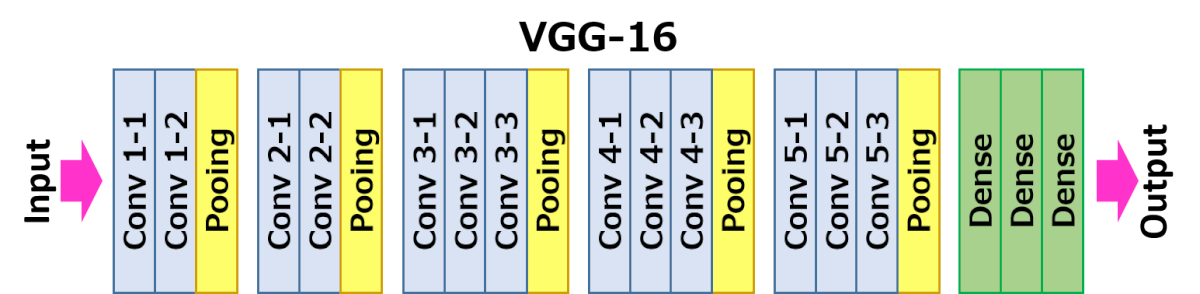
\includegraphics[width=0.8\textwidth]{vgg16.png}
    \caption[VGG16 model]{VGG16 model. Total number of 17 961 168 parameters from convolutional layers can be trained. In order to create transferred model, we need to strip off all Dense layers and add our own. Last Dense layer has to have $N$ amounts of neurons, where $N$ is number of classes. This model was used for ImageNet classification \cite{hassan_2018}.}
    \label{fig:vgg16}
\end{figure}

\begin{figure}
    \centering
    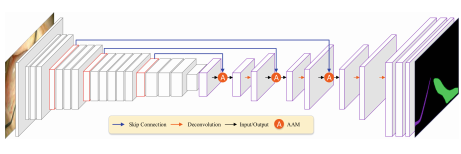
\includegraphics[width=0.8\textwidth]{resnet.PNG}
    \caption[ResNet34 model]{ResNet34 model. This model uses skip connections in order to create deeper model. Because of gradient decay, building and training a deep sequential model is hard, because almost no gradient value propagates to the very first layers \cite{resnet34_model}.}
    \label{fig:resnet_34}
\end{figure}

ResNet, on the other hand, is a much deeper network. My chosen representative architecture, ResNet50, has over 40 of Conv2D layers, and utilizes skip connections in order to have some gradient values in first layers. This enabled creation of much deeper network. Model of smaller model, ResNet34 can be seen in Figure \ref{fig:resnet_34}. VGG16, with one Dense layer with 128 neurons, was chosen as a baseline model. This will help later with hyperparameter tuning since improvements can be seen in the form of better accuracy. 

\subsection{Binary classification}\label{sec:binary_classification}
The first task was to train a model that could only detect failures. This ends up with two classes, defect and healthy. The dataset being almost balanced between both classes helped. VGG16, with one hidden Dense layer, managed to learn 97\% accuracy on test data. When fitting, 30 epochs were passed as a parameter, but learning stopped at the eighth epoch because of Early Stopping. Confusion matrix for this model can be seen in Figure \ref{fig:binary_confusion}. After some hyperparameter tuning, I discovered that by using multiple hidden Dense layers together with training, a few last layers of VGG16 gave better results. There were almost half of false\babelhyphen{nobreak}negative hits, meaning that more defects were being caught. This meant around 1\% improvement in accuracy over the test set. The model had two hidden Dense layers with 128 neurons, two hidden Dense with 64 neurons, and trained three convolutional layers of VGG16. This model can be found on the enclosed medium under the name of "BinaryVGGModel.h5". 

\begin{figure}
\subfloat[Base VGG]{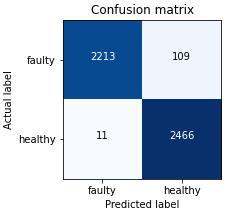
\includegraphics[width = 0.3\textwidth]{BinaryVGGBase.PNG}}
\subfloat[Tuned VGG]{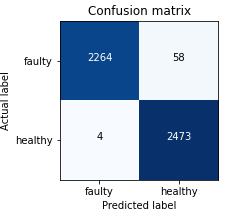
\includegraphics[width = 0.3\textwidth]{BinaryVGGTuned.PNG}}
\subfloat[Tuned ResNet]{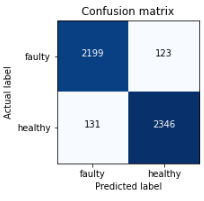
\includegraphics[width = 0.3\textwidth]{BinaryResNetBest.PNG}}
\caption[Confusion matrix comparisson for binary models]{Confusion matrix comparisson for binary models. As can be seen the Tuned VGG model performed the best. } \label{fig:binary_confusion}
\end{figure}
On the other hand, I could not have ResNet50 perform better than VGG16 on the test set. On train set, loss function approached zero, and accuracy was sometimes 100\%, but test set results were around 90-95\%. This is a sign of Overfitting (see Section \ref{sec:overfitting}), but I was not able to not Overfit model and also get better results than with using VGG16. The compared model has three hidden Dense layers with 128 neurons, was trained nine layers deep into ResNet architecture. Training more layers than only those added Dense layers is recommended because the final layers are specifically trained on ImageNet. This means that they are providing different features than those that might be important for this specific purpose. 

\subsection{Categorical classification}
The second task was more challenging. The dataset, as discussed before, contained 16 classes, one for healthy images, and the rest were defect classes. Because the real world does not follow a uniform distribution, defect distribution between defect samples was also not balanced. Another thing was that because of almost a balanced split on the healthy images, this class was suddenly one of the major classes. The other major class was \emph{DEG}, which supposedly means degradation. Degradation of some form can be present in other defects, so this, combined with the fact that \emph{DEG} was a major class in the dataset, meant that some of the images would be classified as this class even if they are labeled as some other different class. Distribution of classes can be seen in Table \ref{tab:class_distribution}. 
\begin{figure}
    \centering
    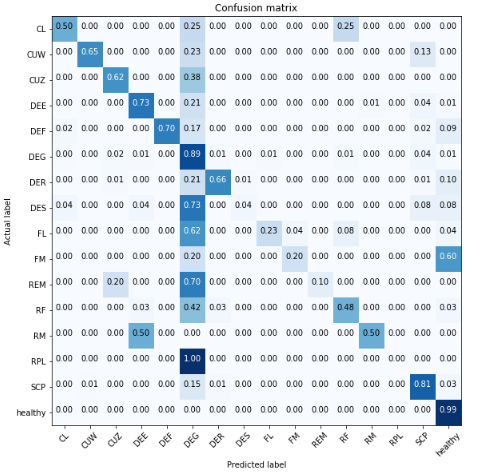
\includegraphics[width=0.8\textwidth]{CategoricalVGGBase.PNG}
    \caption[Confusion matrix of VGG model]{The confusion matrix of base VGG model. In order to better show how well the model did on minor classes, the matrix is normalized. Notice the column of predictions at \emph{DEG}, most of the incorrect predictions were at this category. This label probably means pipe degradation, which could also be present in different labels. You can also see the problem with an unbalanced dataset. This model had 90\% accuracy, which can sound good, but as you can see, most of it is because it can correctly predict healthy images (no canalization defect present) and \emph{DEG} label.}
    \label{fig:categorical_vgg_base}
\end{figure}
\begin{table}[ht!]
    \centering
    \begin{tabular}{|c|c|c|}\hline
        Class Name & \# of images & Percentage\\\hline\hline
        CL      & 8     & 0.16\\\hline
        CUW     & 31    & 0.63\\\hline
        CUZ     & 37    & 0.76\\\hline
        DEE     & 97    & 2.01\\\hline
        DEF     & 53    & 1.09\\\hline
        DEG     & 1588  & 32.77\\\hline
        DER     & 109   & 2.24\\\hline
        DES     & 26    & 0.53\\\hline
        FL      & 26    & 0.53\\\hline
        FM      & 5     & 0.10\\\hline
        REM     & 10    & 0.20\\\hline
        RF      & 33    & 0.68\\\hline
        RM      & 6     & 0.12\\\hline
        RPL     & 1     & 0.02\\\hline
        SCP     & 336   & 6.93\\\hline
        healthy & 2479  & 51.16\\\hline
    \end{tabular}
    \caption[Class distribution]{Class distribution of test set for categorical model. Note that most of classes have representation of less than one percent. This can help model achieve good looking accuracy score but, model fails in classifying minor classes.}
    \label{tab:class_distribution}
\end{table}

Since the previous model showed great results at detecting defects, two experiments are done. First, the dataset will contain all 16 classes to see if one model to rule them all technique can work. In the second experiment, we will assume that the first model high accuracy and could easily find differences between defect and healthy images. This model would be chosen in the first phase, and after that second model would try to classify a given defect. This could eliminate one of the major classes and maybe correctly predict more samples of minor classes.

\begin{figure}
    \centering
    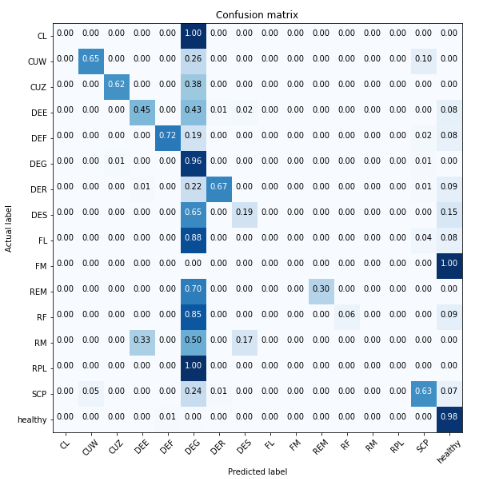
\includegraphics[width=0.8\textwidth]{CategoricalVGGTuned.PNG}
    \caption[Confusion matrix of tuned VGG]{The confusion matrix of best VGG based model. Notice more images flagged as healthy and more images flagged as DEG. 1\% of improvement in accuracy meant significantly worse results on minor classes.}
    \label{fig:categorical_vgg_tuned}
\end{figure}

Lets again, for comparison, create some base model and improve it by adding more Dense layers or mark some inner layers of VGG16 trainable. But first, lets compute parameter \mintinline{python}|class_weights|. This is done using function \mintinline{python}|compute_class_weights()|. The array that this function returns will be passed to \mintinline{python}|fit_generator()| method of the model to further intensify probability, that minor class will not be ignored. But back to training. The base VGG16 model ended up having 91\% accuracy. It finished training after 12 epochs. Confusion matrix of this model can be seen in Figure \ref{fig:categorical_vgg_base}. After giving this base model another hidden Dense layer and allowing it to learn deeper than Dense layers, it improved by 1\%, but this improvement comes with worse spread over minor classes. What is even worse, that there are more false negatives, images classified as healthy, but containing in reality, a canalization defect. The model trained for 14 epochs with 10 layers deep into VGG16 training. Normalized confusion matrix can be seen in Figure \ref{fig:categorical_vgg_tuned}. But again, as for ResNet50, it managed to accomplish at best around 80\%. There will not be a confusion matrix for ResNet since I could not have it surpass VGG in this task.

Since ResNet was bad at both tasks, I have chosen to exclude it from the last test. I also have chosen to only try to create the best model possible. This last experiment assumes that on the input, there are mostly only defect images because binary classification has proven very reliable (see Section \ref{sec:binary_classification}). This, in theory, moves the heavy lifting from the model, which has to decide between 16 classes to binary model. That can lead to around 2\% false negativeness, which comes from the binary model, and according to test data, close to 0\% false positiveness. In theory, we should have a better opportunity to create a better defect classifying model. But first, let's recalculate how well the previous model did without a healthy class, to be able to compare both methods. This is actually easy, as you can see in the equation:

$$acc_n = \frac{y_{correct} - y_{h\_correct}}{n - n_h}$$

where $acc_n$ is accuracy without healthy class, $y_{h\_correct}$ is number of correctly predicted healthy samples, $n$ is number of test samples and $n_h$ is size of healthy class. Because there were no exact numbers provided in this thesis, following estimate equation will be used for recalculation:

$$acc_{n} = \frac{(acc \times n) - (acc_h \times n_h)}{n - n_{h}}$$

\begin{figure}
    \centering
    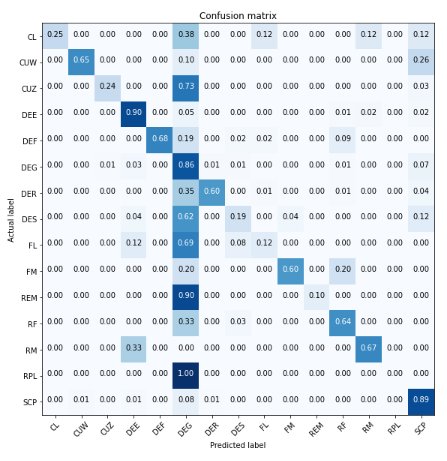
\includegraphics[width=.8\textwidth]{CategoricalVGGTwoModels.PNG}
    \caption[Confusion matrix of model trained only on defect images]{Confusion matrix of model trained only on defect images. Misclassification as DEG is still present but minor classes start to have greater presence on diagonal (correctly classified). }
    \label{fig:categorical_combination}
\end{figure}

where $acc$ model accuracy and $acc_h$ is accuracy for a healthy class. This is only an estimate, there will be rounding error, but it will not be significant enough to matter. Substituting into the equation, resulting accuracy of the model, if a healthy class is not taken into account, is around 84.5\%. Also, it should be mentioned that now the dominant class \emph{DEG} takes 67\% of the dataset. So let's train a new model on the reduced dataset and compare those two methods. The model took 26 epochs to train. The learning rate was adjusted to $1 \times 10^{-4}$, and the model had 3 Dense layers, training 9 layers deep into convolutional layers. The resulting accuracy was 87\%, which is at least 2\% improvement in accuracy, confusion matrix can be seen in Figure \ref{fig:categorical_combination}. This combination proved to be a better method than the one model method. Because of this, I would suggest combining two models. The model can be found on the enclosed medium under the name of "categorical-combination.h5".

\begin{conclusion}
    The main goal of this thesis was to create a convolutional neural network with high precision of detecting failures. The created network has very high precision at detecting failures. It can also point out which failure might have occurred, but it is not very efficient at this yet, mainly in minor classes. This could be a subject of further work, or the net could be deployed with active learning. Also, failure segmentation could be another topic of further work.
\end{conclusion}

% \bibliographystyle{csn690}
% \bibliography{mybibliographyfile}

% \sloppy
\emergencystretch 4em
\printbibliography
\fussy

\appendix

% \printglossaries
\printnoidxglossary[type=\acronymtype,numberedsection=autolabel] % glossaries

\chapter{Content of enclosed medium}\label{app:CD_content}

%upravte podle skutecnosti

\begin{figure}
    \dirtree{%
        .1 models\DTcomment{trained models}.
        .1 src.
        .2 notebooks\DTcomment{jupyter notebooks}.
        .2 thesis\DTcomment{source code of the thesis in \LaTeX{}}.
        .1 text.
        .2 thesis.pdf\DTcomment{thesis text in PDF}.
    }
\end{figure}

\end{document}
